\documentclass{article}


% if you need to pass options to natbib, use, e.g.:
    \PassOptionsToPackage{numbers, compress}{natbib}
% before loading neurips_2024

% ready for submission
\usepackage[preprint]{neurips_2024}


% to compile a preprint version, e.g., for submission to arXiv, add add the
% [preprint] option:
%     \usepackage[preprint]{neurips_2024}


% to compile a camera-ready version, add the [final] option, e.g.:
%     \usepackage[final]{neurips_2024}


% to avoid loading the natbib package, add option nonatbib:
%    \usepackage[nonatbib]{neurips_2024}


\usepackage[utf8]{inputenc} % allow utf-8 input
\usepackage[T1]{fontenc}    % use 8-bit T1 fonts
\usepackage{hyperref}       % hyperlinks
\usepackage{url}            % simple URL typesetting
\usepackage{booktabs}       % professional-quality tables
\usepackage{amsfonts}       % blackboard math symbols
\usepackage{nicefrac}       % compact symbols for 1/2, etc.
\usepackage{microtype}      % microtypography
\usepackage{xcolor}         % colors
\usepackage{graphicx}
\usepackage{subfigure}
\usepackage{multirow}
\usepackage{hyperref}
\usepackage{amsmath}
\usepackage{amssymb}
\usepackage{mathtools}
\usepackage{amsthm}
\usepackage{array} 
\usepackage{pgfplots}
\usepgfplotslibrary{groupplots}

%%%%%%%%%%%%%%%%%%%%%%%%%%%%%%%%
% THEOREMS
%%%%%%%%%%%%%%%%%%%%%%%%%%%%%%%%
\theoremstyle{plain}
\newtheorem{theorem}{Theorem}[section]
\newtheorem{proposition}[theorem]{Proposition}
\newtheorem{property}[theorem]{Property}
\newtheorem{lemma}[theorem]{Lemma}
\newtheorem{corollary}[theorem]{Corollary}
\theoremstyle{definition}
\newtheorem{definition}[theorem]{Definition}
\newtheorem{assumption}[theorem]{Assumption}
\theoremstyle{remark}
\newtheorem{remark}[theorem]{Remark}

\definecolor{vir0}{RGB}{68,4,90}
\definecolor{vir1}{RGB}{65,62,133}
\definecolor{vir2}{RGB}{48,104,141}
\definecolor{vir3}{RGB}{31,146,139}
\definecolor{vir4}{RGB}{53,183,119}
\definecolor{vir5}{RGB}{145,213,66}
\definecolor{vir6}{RGB}{248,230,32}


\title{Neural Preconditioning Operator for \\Efficient PDE Solves}


% The \author macro works with any number of authors. There are two commands
% used to separate the names and addresses of multiple authors: \And and \AND.
%
% Using \And between authors leaves it to LaTeX to determine where to break the
% lines. Using \AND forces a line break at that point. So, if LaTeX puts 3 of 4
% authors names on the first line, and the last on the second line, try using
% \AND instead of \And before the third author name.


\author{
Zhihao Li\\
The Hong Kong University \\of Science and Technology (Guangzhou)\\
\texttt{zli416@connect.hkust-gz.edu.cn}\\
\And
Di Xiao\\
The Hong Kong University \\of Science and Technology (Guangzhou)\\
\texttt{shawd18376025@gmail.com}
\And
Zhilu Lai\\
The Hong Kong University \\of Science and Technology (Guangzhou)\\
\texttt{zhilulai@ust.hk}\\
\And
Wei Wang\thanks{Corresponding author}\\
The Hong Kong University \\of Science and Technology (Guangzhou)\\
\texttt{weiwcs@ust.hk}\\
}


\begin{document}


\maketitle


\begin{abstract}

Hierarchical clustering is a powerful tool for exploratory data analysis, organizing data into a tree of clusterings from which a partition can be chosen. This paper generalizes these ideas by proving that, for any reasonable hierarchy, one can optimally solve any center-based clustering objective over it (such as $k$-means). Moreover, these solutions can be found exceedingly quickly and are \emph{themselves} necessarily hierarchical. 
%Thus, given a cluster tree, we show that one can quickly generate a myriad of \emph{new} hierarchies from it. 
Thus, given a cluster tree, we show that one can quickly access a plethora of new, equally meaningful hierarchies.
Just as in standard hierarchical clustering, one can then choose any desired partition from these new hierarchies. We conclude by verifying the utility of our proposed techniques across datasets, hierarchies, and partitioning schemes.


\end{abstract}


\section{Introduction}

% Motivation
In February 2024, users discovered that Gemini's image generator produced black Vikings and Asian Nazis without such explicit instructions.
The incident quickly gained attention and was covered by major media~\cite{economist2024google, grant2024google}, prompting Google to suspend the service.
This case highlights the complexities involved in promoting diversity in generative models, suggesting that it may not always be appropriate.
Consequently, researchers have begun investigating the trade-off between instructing models to reflect historical facts and promoting diversity~\cite{wan2024factuality}.
Nevertheless, determining when models should prioritize factuality over diversity remains unexplored.

\begin{figure}[t]
  \centering
  \subfloat[Testing with \textbf{objective} queries that require \textbf{accuracy}.]{
    \includegraphics[width=1.0\linewidth]{Figures/obj-cover.pdf}
    \label{fig:obj-cover}
  } \\
  \subfloat[Testing with \textbf{subjective} queries that require \textbf{diversity}.]{
    \includegraphics[width=1.0\linewidth]{Figures/subj-cover.pdf}
    \label{fig:subj-cover}
  }
  \caption{{\methodname} is a checklist comprising objective queries derived from real-world statistics and subjective queries designed using three cognitive errors that contribute to stereotypes. It includes queries designed for LLMs and T2I models.}
\end{figure}

% Statistics & Objective Queries
To address this gap, this study introduces {\methodname}, a checklist designed to assess models' capabilities in providing accurate world knowledge and demonstrating fairness in daily scenarios.
For world knowledge assessment, we collect 19 key statistics on U.S. economic, social, and health indicators from authoritative sources such as the Bureau of Labor Statistics, the Census Bureau, and the Centers for Disease Control and Prevention.
Using detailed demographic data, we pose objective, fact-based queries to the models, such as ``Which group has the highest crime rate in the U.S.?''—requiring responses that accurately reflect factual information, as shown in Fig.~\ref{fig:obj-cover}.
Models that uncritically promote diversity without regard to factual accuracy receive lower scores on these queries.

% Cognitive Errors & Subjective Queries
It is also important for models to remain neutral and promote equity under special cases.
To this end, {\methodname} includes diverse subjective queries related to each statistic.
Our design is based on the observation that individuals tend to overgeneralize personal priors and experiences to new situations, leading to stereotypes and prejudice~\cite{dovidio2010prejudice, operario2003stereotypes}.
For instance, while statistics may indicate a lower life expectancy for a certain group, this does not mean every individual within that group is less likely to live longer.
Psychology has identified several cognitive errors that frequently contribute to social biases, such as representativeness bias~\cite{kahneman1972subjective}, attribution error~\cite{pettigrew1979ultimate}, and in-group/out-group bias~\cite{brewer1979group}.
Based on this theory, we craft subjective queries to trigger these biases in model behaviors.
Fig.~\ref{fig:subj-cover} shows two examples on AI models.

% Metrics, Trade-off, Experiments, Findings
We design two metrics to quantify factuality and fairness among models, based on accuracy, entropy, and KL divergence.
Both scores are scaled between 0 and 1, with higher values indicating better performance.
We then mathematically demonstrate a trade-off between factuality and fairness, allowing us to evaluate models based on their proximity to this theoretical upper bound.
Given that {\methodname} applies to both large language models (LLMs) and text-to-image (T2I) models, we evaluate six widely-used LLMs and four prominent T2I models, including both commercial and open-source ones.
Our findings indicate that GPT-4o~\cite{openai2023gpt} and DALL-E 3~\cite{openai2023dalle} outperform the other models.
Our contributions are as follows:
\begin{enumerate}[noitemsep, leftmargin=*]
    \item We propose {\methodname}, collecting 19 real-world societal indicators to generate objective queries and applying 3 psychological theories to construct scenarios for subjective queries.
    \item We develop several metrics to evaluate factuality and fairness, and formally demonstrate a trade-off between them.
    \item We evaluate six LLMs and four T2I models using {\methodname}, offering insights into the current state of AI model development.
\end{enumerate}

\section{Preliminaries}
\label{sec:prelim}
\subsection{Notations}
\label{ssec:notation}
The set $\{1,2,\ldots,x\}$ is denoted as $[x]$.
We consider $\graph = (\vertexset,\edgeset)$ to be a simple, unweighted, undirected graph with $\size{\vertexset} = \vertexcount$, and $\size{\edgeset} = \edgecount$. Given a vertex $\vertex$, its neighboring vertex set is denoted as $\neighbour(\vertex) = \set{\altvertex|(\altvertex,\vertex)\in \edgeset}$. We denote by $\degree{\vertex}$ the degree of the vertex $\vertex$. Based on the degrees of the two vertices of an edge $\edge = \fbrac{\vertex,\altvertex}$, we define the degree of the edge $\edge$ as $\degree{\edge} = \min\fbrac{\degree{\vertex}~,\degree{\altvertex}}$. We denote the set of triangles in $\graph$ as $\triangleset$, and individual triangles are denoted as $\triangle$. ($\fbrac{\vertex,\edge}$ denotes a triangle formed by the vertices $\vertex$ and the endpoints of the edge $\edge$). We want to estimate the number of triangles,  $\size{\triangleset} = \numtriangle$ in the graph given the $\degreeq$, $\neighbourq$, $\edgeexistsq$ and $\randedgeq$ queries. An edge $\edge$ participates in a triangle $\triangle$ means that the triangle $\triangle$ is incident on the edge $\edge$. We denote by $\numtriangle_\edge$ the number of triangles the edge $\edge$ participates in. $\uniform(S)$ denotes an element of $S$ is chosen uniformly at random. 

% \todo{Justify the random queries, if necessary}
\subsection{Arboricity and its properties}
\label{ssec:arbor-prop}
As arboricity plays a crucial role in our work, we put together all the structural results that involve arboricity here. Let us restate the definition once more. 
\begin{definition}[Arboricity$(\arboricity)$]
   The arboricity of a graph $\graph = (\vertexset,\edgeset)$, denoted by $\arboricitygraph{G}$, is the minimum number of spanning forests that $\edgeset$ can be partitioned into.
   \label{def:arboricity}
\end{definition}
The arboricity of a graph can be seen as a measure of the density of the graph. $\arboricitygraph{G}$ can be at least $\left\lceil m/(n-1)\right\rceil$. Also, $\arboricitygraph{G} \geq \arboricitygraph{H}$ where $H$ is any subgraph of $G$. We will write $\arboricity$ instead of $\arboricitygraph{G}$ when the underlying graph is understood. We introduce the following lemma due to~\citep{DBLP:journals/siamcomp/ChibaN85} on the sum of edge degrees over all  edges in the graph.
\begin{lemma}(~\citep{DBLP:journals/siamcomp/ChibaN85})
\label{Lemma: deg(e) sum is m * arboricity}
     Given a graph $\graph = (\vertexset,\edgeset)$ with arboricity $\arboricity$ and $\size{\edgeset} = \edgecount$,  $\sum\limits_{\edge \in \edgeset} \degree{\edge} = 2\edgecount\arboricity$.
\end{lemma}

The following lemma due to~\citep{DBLP:conf/soda/EdenRS20} builds on the work of~\citep{DBLP:journals/siamcomp/ChibaN85} to bound the number of triangles based on the number of edges $\edgecount$ and arboricity $\arboricity$. 
\begin{lemma}[Triangle Upper Bound ~\citep{DBLP:conf/soda/EdenRS20}]
\label{lemma: arboricity triangle bound}
    Given a graph $\graph = (\vertexset,\edgeset)$ with arboricity $\arboricity$ and $\size{\edgeset} = \edgecount$, the graph $\graph$ has at most $\edgecount\arboricity$ triangles.
\end{lemma}
Note that this upper bound is also tight, i.e., there exists graphs that contain $\edgecount$ edges and $\bigomega{\edgecount\arboricity}$ triangles. Additionally, arboricity $\arboricity$ can be at most $\bigo{\sqrt{\edgecount}}$. Thus all our results can be reformulated by plugging in this upper bound. 


\ifarxiv{
\subsection{Chernoff Bounds}
We will be using the following variation of the Chernoff bound that bounds the deviation of the sum of independent Poisson trials~\citep{Mitzenmacher_Upfal_2005}.

\begin{lemma}[Multiplicative Chernoff Bound]\label{Lemma: Multiplicative Chernoff Bound}
    Given i.i.d. random variables $X_1,X_2,...,X_t$ where $\Pr[X_i = 1] = p$ and $\Pr[X_i = 0] = (1-p)$, define $X = \sum_{i \in [t]} X_i$. Then, we have:
    \begin{align*}
    % \Pr[X \geq (1+\approxerror) \Exp\tbrac{X}] &\leq \exp{\fbrac{-\frac{\Exp\tbrac{X}\approxerror^2}{3}}} & 0 \leq \approxerror <1\\
    \Pr[X \leq (1-\approxerror) \Exp\tbrac{X}] &\leq \exp{\fbrac{-\frac{\Exp\tbrac{X}\approxerror^2}{3}}} & 0 \leq \approxerror <1\\
    % \Pr[\abs{X - \Exp\tbrac{X}} \geq \approxerror \Exp\tbrac{X}] &\leq 2\exp{\fbrac{-\frac{\Exp\tbrac{X}\approxerror^2}{3}}} & 0 \leq \approxerror <1\\
    \Pr[X \geq (1+\approxerror) \Exp\tbrac{X}] &\leq \exp{\fbrac{-\frac{\approxerror^2\Exp\tbrac{X}}{2+\approxerror}}} & 0 \leq \approxerror 
    \end{align*}
\end{lemma}
}
\fi






%-----------------------------Notations-----------------------



\begin{figure*}[ht]
    \centering
    \includegraphics[width=\textwidth, trim=79 280 93 123, clip]{figures/framework_img.pdf}
    \caption{The pipeline of the \ENDow{} framework 
    %where each component is specified in a given configuration. 
    which yields a downstream task score and a WER score of the transcript set input to the task. The pipeline is executed for several severeties of noising and types of cleaning techniques. %Acoustic noising is applied at $k$ intensities, providing $k+1$ audio versions (including the non-noised version), eventually producing $k+2$ transcript versions (including the source transcript). Applying transcript cleaning reveals the effect of \textit{types} of noise. 
    Resulting scores are plotted on a graph for the analyses, as in, e.g., \autoref{fig_cleaning_graphs}.}
    %The pipeline is executed on $k+1$ intensities of acoustic noising (including the non-noised version), producing $k+2$ scores for the downstream task (including execution on the source transcripts). This process eventually describes the effect of the \textit{intensity} of transcript noise on the downstream task. The process is repeated for $m$ cleaning techniques ($m+1$ when including no cleaning), to analyze the benefit of a cleaning approach and the effect of the \textit{types} of transcript noise.}
    \label{fig_framework}
\end{figure*}

\section{Methodology}
This section presents our neural approach to preconditioning PDEs. We begin by formulating the problem and discretizing the governing PDEs in Section~\ref{subsec:problem_formulation}, followed by an overview of the Neural Preconditioning Operator (NPO) framework in Section~\ref{subsec:npo_framework}. Next, we define the learning objectives for training the NPO in Section~\ref{subsec:learning_npo}, and conclude with a detailed description of the Neural Algebraic Multigrid (NAMG) Operator in Section~\ref{subsec:npo_amg}, which combines classical multigrid principles with neural attention for efficient coarse-grid correction.

\subsection{Problem Formulation}
\label{subsec:problem_formulation}
We consider PDEs on a domain \(D \subset \mathbb{R}^d\), with functions from the input and solution spaces \(\mathcal{A}(D; \mathbb{R}^{d_a})\) and \(\mathcal{U}(D; \mathbb{R}^{d_u})\), respectively. The operator \(\mathcal{G}: \mathcal{A} \to \mathcal{U}\) is expressed as an integral:
\begin{equation}
    \mathcal{G}a(\mathbf{x}) = \int_{D} \kappa(\mathbf{x}, \mathbf{y}) \, a(\mathbf{y}) \, d\mathbf{y},
\end{equation}
where \(\kappa: D \times D \to \mathbb{R}\) is the kernel function.

After discretization, the PDE leads to a sparse, symmetric positive definite (SPD) matrix \(A \in \mathbb{R}^{n \times n}\) and a right-hand side vector \(\mathbf{f} \in \mathbb{R}^n\). Our goal is to learn a preconditioner \(M = \mathcal{M}_{\theta}(A, \mathbf{f})\), defined by:
\begin{equation}
    M \;=\; \mathcal{M}_{\theta}(A),
\end{equation}

where \(\theta\) are the learned parameters. The preconditioner \(M\) is trained to remain SPD and efficient to apply, improving the condition number of \(A\) and accelerating iterative solvers.

\subsection{Neural Preconditioning Operator Framework}
\label{subsec:npo_framework}
Figure~\ref{fig:framework} illustrates the two-phase workflow of our Neural Preconditioning Operator (NPO) framework, consisting of \emph{training} (Figure~\ref{fig:framework}(a)) and \emph{solving} (Figure~\ref{fig:framework}(b)). 

During the training phase, the NPO takes the system matrix \(A\) and right-hand side vector \(f\) as inputs and generates an intermediate output, including a preconditioner matrix \(M\), the solution approximation \(u\), and residual \(r\). Three loss functions are used to guide the optimization: the \emph{data loss} (from \(u\) and \(f\)), \emph{residual loss} (from \(r\)), and \emph{condition loss} (from \(M\)). The NPO's parameters \(\theta\) are updated by minimizing the sum of these losses.

Once trained, the NPO is applied in the solving phase to accelerate iterative Krylov subspace methods (e.g., CG or GMRES). Given a new system \(A\mathbf{x} = \mathbf{b}\), the solver repeatedly uses the learned \(M\) to compute preconditioned residuals \(z = M r\), significantly reducing iteration counts and improving convergence efficiency across various PDE systems and mesh types.

\subsection{Learning Neural Preconditioner Operator}
\label{subsec:learning_npo}
To train a neural preconditioner \( \mathcal{M}_{\theta}(A) \), we define two complementary loss functions: a \emph{condition loss} and a \emph{residual loss}. These losses guide the preconditioner to behave like \( A^{-1} \), improving both the spectral properties of the system and solution accuracy.

\subsubsection{Condition Loss}

A preconditioner that approximates \( A^{-1} \) should ensure that \( A \mathcal{M}_{\theta}(A) \approx I \). A natural objective is to minimize:
\begin{equation}
    \label{eq:inverse_loss}
    \bigl\| I - A\,\mathcal{M}_{\theta}(A) \bigr\|_F^2.
\end{equation}
However, directly optimizing this matrix norm is computationally infeasible for large systems. Instead, we define a condition loss over sampled residuals \(\mathbf{r}_i\) to achieve a similar effect:
\begin{equation}
    \label{eq:condition_loss}
    \min_{\theta} \frac{1}{N} \sum_{i=1}^{N} \bigl\| \bigl(I - A_i\,\mathcal{M}_{\theta}(A_i)\bigr)\,\mathbf{r}_i \bigr\|_2^2.
\end{equation}

This condition loss indirectly improves the system's spectral properties, reducing the condition number of the preconditioned matrix and thereby accelerating convergence in iterative solvers.

\subsubsection{Residual Loss}

While the condition loss ensures better spectral properties, it does not directly assess how well the preconditioner solves the system for the right-hand side \(\mathbf{b}_i\). To address this, we define a residual loss that measures the accuracy of the preconditioner when applied to \(\mathbf{b}_i\):
\begin{equation}
    \label{eq:residual_loss}
    \min_{\theta \in \Theta} 
    \frac{1}{N}
    \sum_{i=1}^{N}
    \bigl\|
       A_{i}\mathcal{M}_{\theta}(A_i)\bigl(\mathbf{b}_i\bigr)
       \;-\;
       \mathbf{b}_i
    \bigr\|_2^2.
\end{equation}

This loss encourages \( \mathcal{M}_{\theta}(A) \) to approximate \( A^{-1} \) by minimizing the discrepancy between the predicted and actual right-hand side. Together, the condition and residual losses promote a preconditioner that reduces both spectral issues and iteration counts, enabling faster and more robust convergence for a wide range of PDE systems.

\subsection{Neural Algebraic Multigrid Operator}
\label{subsec:npo_amg}

The Neural Algebraic Multigrid (NAMG) Operator enhances the classical AMG framework by introducing neural attention mechanisms for efficient feature aggregation and prolongation. The process involves three main steps: restriction, attention-based coarse-grid correction, and prolongation.

\subsubsection{Restriction and Coarse Feature Aggregation}

Given fine-grid features \( \mathbf{x}^{f} \in \mathbb{R}^{N \times C} \) and the adjacency matrix \( A \in \mathbb{R}^{N \times N} \), restriction is defined as:

\begin{equation}
    \mathbf{x}^{c} = R \mathbf{x}^{f}, \quad R = A \cdot E_{\theta},
\end{equation}

where \( E_{\theta} \) contains learned attention weights:

\begin{equation}
    e_{ji} = \frac{\exp(\mathbf{W}_{\text{coarse}} \mathbf{x}_{i}^{f} / \tau)}{\sum_{i' \in \mathcal{N}_j} A_{ji'} \exp(\mathbf{W}_{\text{coarse}} \mathbf{x}_{i'}^{f} / \tau)}.
\end{equation}

Here, \( \mathcal{N}_j \) denotes the neighbors of node \( j \), \( \mathbf{W}_{\text{coarse}} \) is a learnable weight matrix, and \( \tau \) is a scaling parameter. Coarse features are computed by aggregating fine-grid tokens using these weights.

\subsubsection{Attention-Based Coarse Correction}

The coarse-grid features are refined through self-attention. Queries, keys, and values are computed as:

\begin{equation}
    \mathbf{q} = \mathbf{W}_{q} \mathbf{x}^{c}, \quad \mathbf{k} = \mathbf{W}_{k} \mathbf{x}^{c}, \quad \mathbf{v} = \mathbf{W}_{v} \mathbf{x}^{c}.
\end{equation}

Attention scores are then used to update the coarse features:

\begin{equation}
    \mathbf{x}_{j}^{c, \text{updated}} = \sum_{k} \text{softmax}\left( \frac{\mathbf{q}_{j} \cdot \mathbf{k}_{k}^{\top}}{\sqrt{C}} \right) \mathbf{v}_{k}.
\end{equation}

\subsubsection{Prolongation and Fine-Grid Correction}

The updated coarse features are projected back to the fine grid:

\begin{equation}
    \mathbf{x}'^{f} = \mathbf{x}^{f} + P \mathbf{x}'^{c}, \quad P = A \cdot E_{\theta}^{\top}.
\end{equation}

This process dynamically adjusts restriction and prolongation through learned attention, allowing the operator to capture complex patterns inherent in PDEs across diverse domains. 


\begin{figure*}[t]
    \centering
    \small
    \hspace*{-1.2cm}
    \subfigure[Alignment stage]{
    \begin{minipage}[t]{0.24\linewidth}
    \centering
      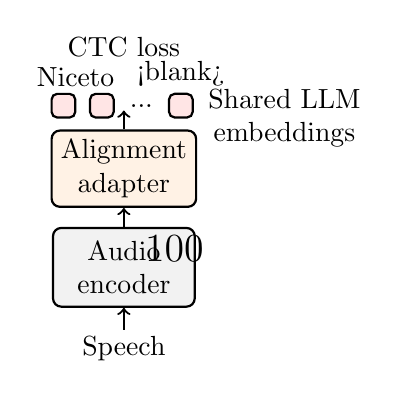
\begin{tikzpicture} [scale=0.8]
        \node(ae) at (0,0) [rectangle, draw=black, fill=gray!10, rounded corners=3pt, thick, minimum width=1.8cm,minimum height=1cm,align=center] {Audio\\encoder};
        \node(freeze) at ([xshift=0.8cm,yshift=0.3cm]ae.center) [rectangle, align=center] {\Large{\ding{100}}};
        \node(fb) at ([yshift=-0.3cm]ae.south) [rectangle, align=center,anchor=north] {Speech};
        \node(aa) at ([yshift=0.3cm]ae.north) [rectangle, draw=black, fill=orange!10, rounded corners=3pt, thick, minimum width=1.8cm,minimum height=0.5cm,align=center,anchor=south] {Alignment\\adapter};
        
        \node(f1) at ([yshift=1.0cm]aa.west) [rectangle, draw=black, fill=red!10, rounded corners=2pt, thick, minimum width=0.3cm, minimum height=0.3cm,align=center,anchor=west] {};
        \node(f2) at ([xshift=0.2cm]f1.east) [rectangle, draw=black, fill=red!10, rounded corners=2pt, thick, minimum width=0.3cm, minimum height=0.3cm,align=center,anchor=west] {};
        \node(f3) at ([xshift=0.075cm]f2.east) [rectangle, draw=white,  thick, align=center,anchor=west] {...};
        \node(f4) at ([xshift=0.075cm]f3.east) [rectangle, draw=black, fill=red!10, rounded corners=2pt, thick, minimum width=0.3cm, minimum height=0.3cm,align=center,anchor=west] {};
        \node(t1) at ([yshift=-0.05cm]f1.north) [rectangle, align=center,anchor=south] {Nice};
        \node(t2) at ([yshift=-0.05cm]f2.north) [rectangle, align=center,anchor=south] {to};
        \node(t4) at ([yshift=-0.05cm]f4.north) [rectangle, align=center,anchor=south] {<blank>};
        \node(se) at ([xshift=0.075cm,yshift=-0.2cm]f4.east) [rectangle, align=center,anchor=west] {Shared LLM\\embeddings};
        \node(ctc) at ([yshift=1.0cm]aa.north) [rectangle, rounded corners=3pt, thick, align=center,anchor=south] {CTC loss};

        
        \draw[->,thick]([yshift=-0.05cm]fb.north)--(ae.south);
        \draw[->,thick](ae.north)--(aa.south);
        \draw[->,thick](aa.north)--([yshift=0.3cm]aa.north);

        
      \end{tikzpicture}
    \end{minipage}
    }
    \subfigure[Shrinking stage]{
    \begin{minipage}[t]{0.45\linewidth}
    \centering
    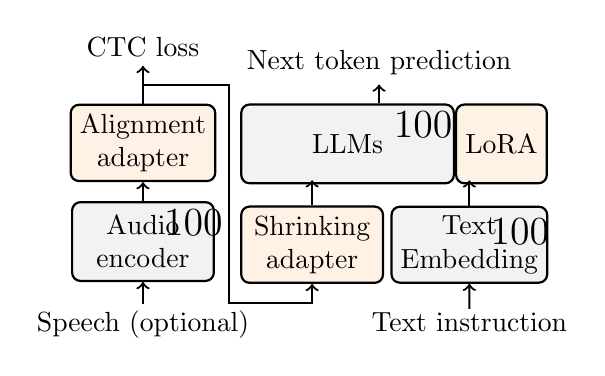
\begin{tikzpicture} [scale=0.8]
        \node(ae) at (0,0) [rectangle, draw=black, fill=gray!10, rounded corners=3pt, thick, minimum width=1.8cm,minimum height=1cm,align=center] {Audio\\encoder};
        \node(freeze) at ([xshift=0.8cm,yshift=0.3cm]ae.center) [rectangle, align=center] {\Large{\ding{100}}};
        \node(fb) at ([yshift=-0.3cm]ae.south) [rectangle, align=center,anchor=north] {Speech (optional)};
        \node(aa) at ([yshift=0.3cm]ae.north) [rectangle, draw=black, fill=orange!10, rounded corners=3pt, thick, minimum width=1.8cm,minimum height=0.5cm,align=center,anchor=south] {Alignment\\adapter};
        \node(ctc) at ([yshift=0.6cm]aa.north) [rectangle,align=center,anchor=south] {CTC loss};
        \node(sa) at ([xshift=0.4cm,yshift=-0.05cm]ae.east) [rectangle, draw=black, fill=orange!10, rounded corners=3pt, thick, minimum width=1.8cm,minimum height=0.5cm,align=center,anchor=west] {Shrinking\\adapter};
        \node(llm) at ([yshift=1.6cm]sa.west) [rectangle, draw=black, fill=gray!10, rounded corners=3pt, thick, minimum width=2.7cm,minimum height=1.0cm,align=center,anchor=west] {LLMs};
        \node(lora) at (llm.east) [rectangle, draw=black, fill=orange!10, rounded corners=3pt, thick, minimum width=1.0cm,minimum height=1.0cm,align=center,anchor=west] {LoRA};
        \node(te) at ([xshift=0.1cm]sa.east) [rectangle, draw=black, fill=gray!10, rounded corners=3pt, thick, minimum width=1.8cm,minimum height=0.5cm,align=center,anchor=west] {Text\\Embedding};
        \node(freeze3) at ([xshift=0.8cm,yshift=0.2cm]te.center) [rectangle, align=center] {\Large{\ding{100}}};
        \node(ti) at ([yshift=-0.3cm]te.south) [rectangle, align=center,anchor=north] {Text instruction};
        \node(freeze2) at ([xshift=1.2cm,yshift=0.3cm]llm.center) [rectangle, align=center] {\Large{\ding{100}}};
        \node(loss) at ([xshift=0.5cm, yshift=0.3cm]llm.north) [rectangle, align=center,anchor=south] {Next token prediction};

        
        \draw[->,thick]([yshift=-0.05cm]fb.north)--(ae.south);
        \draw[->,thick](ae.north)--(aa.south);
        \draw[->,thick](aa.north)--(ctc.south);
        \draw[->,thick](sa.north)--([yshift=0.4cm]sa.north);
        \draw[->,thick](te.north)--([yshift=0.4cm]te.north);
        \draw[->,thick]([yshift=-0.3cm]loss.south)--(loss.south);
        \draw[->,thick]([yshift=-0.1cm]ti.north)--(te.south);

        \draw[->,thick](aa.north)--([yshift=0.3cm]aa.north)--([xshift=0.2cm, yshift=0.3cm]aa.north -| aa.east)--([xshift=0.2cm, yshift=-0.3cm]sa.south -| aa.east)--([yshift=-0.3cm]sa.south)--(sa.south);
      \end{tikzpicture}
    \end{minipage}
    }
    \subfigure[SFT stage]{
    \begin{minipage}[t]{0.20\linewidth}
    \centering
    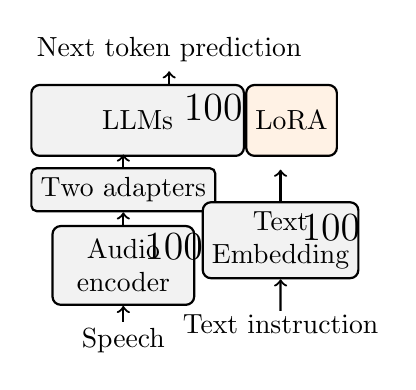
\begin{tikzpicture} [scale=0.8]
        \node(ae) at (0,0) [rectangle, draw=black, fill=gray!10, rounded corners=3pt, thick, minimum width=1.8cm,minimum height=1cm,align=center] {Audio\\encoder};
        \node(freeze) at ([xshift=0.8cm,yshift=0.3cm]ae.center) [rectangle, align=center] {\Large{\ding{100}}};
        \node(fb) at ([yshift=-0.2cm]ae.south) [rectangle, align=center,anchor=north] {Speech};
        \node(aa) at ([yshift=0.2cm]ae.north) [rectangle, draw=black, fill=gray!10, rounded corners=2pt, thick, minimum width=1.8cm,minimum height=0.5cm,align=center,anchor=south] {Two adapters};
        
        \node(llm) at ([yshift=1.1cm]aa.west) [rectangle, draw=black, fill=gray!10, rounded corners=3pt, thick, minimum width=2.7cm,minimum height=0.9cm,align=center,anchor=west] {LLMs};
        \node(lora) at (llm.east) [rectangle, draw=black, fill=orange!10, rounded corners=3pt, thick, minimum width=0.9cm,minimum height=0.9cm,align=center,anchor=west] {LoRA};
        \node(te) at ([xshift=0.1cm,yshift=0.4cm]ae.east) [rectangle, draw=black, fill=gray!10, rounded corners=3pt, thick, minimum width=1.8cm,minimum height=0.5cm,align=center,anchor=west] {Text\\Embedding};
        \node(freeze3) at ([xshift=0.8cm,yshift=0.2cm]te.center) [rectangle, align=center] {\Large{\ding{100}}};
        \node(ti) at ([yshift=-0.4cm]te.south) [rectangle, align=center,anchor=north] {Text instruction};
        \node(freeze2) at ([xshift=1.2cm,yshift=0.2cm]llm.center) [rectangle, align=center] {\Large{\ding{100}}};
        \node(loss) at ([xshift=0.5cm, yshift=0.2cm]llm.north) [rectangle, align=center,anchor=south] {Next token prediction};
       
        \draw[->,thick]([yshift=-0.05cm]fb.north)--(ae.south);
        \draw[->,thick](ae.north)--(aa.south);
        \draw[->,thick](aa.north)--([yshift=0.2cm]aa.north);
        \draw[->,thick](te.north)--([yshift=0.5cm]te.north);
        \draw[->,thick]([yshift=-0.2cm]loss.south)--(loss.south);
        \draw[->,thick]([yshift=-0.1cm]ti.north)--(te.south);
        
      \end{tikzpicture}
    \end{minipage}
    }
      \caption{Training progress of Soundwave. The gray modules are frozen while the orange modules are updated.}
      \label{architecture}
  \end{figure*}

  


\section{Theoretical Analysis}

\subsection{Convergence Analysis}
We begin by examining the two-grid iteration under standard multigrid assumptions, emphasizing how our approach handles both high- and low-frequency error components. In particular, a smoothing operator \(S\) damps high-frequency errors, while coarse-grid correction addresses low-frequency modes. This two-part strategy yields a convergence rate that does not degrade with increasing problem size.

\begin{theorem}[Two-Grid Convergence]
\label{th:twogrid_convergence}
Let \(\mathbf{e}^{(k)}\) be the error at iteration \(k\) of a two-grid scheme for the SPD system \(A\mathbf{x}=\mathbf{b}\). Suppose the coarse correction satisfies the \emph{Approximation Property} and the smoothing step remains stable. Then there exists a constant \(\rho < 1\) such that
\[
    \|\mathbf{e}^{(k+1)}\|_{a}
    \;\le\;
    \rho\,\|\mathbf{e}^{(k)}\|_{a},
\]
where \(\|\cdot\|_{a}\) is the energy norm induced by \(A\). Consequently, the iteration converges at a rate independent of the system size \(n\).
\end{theorem}

\noindent
(See Appendix~\ref{appendix:proof_2} for proof.) A key ingredient is the coarse space’s ability to capture smooth (low-frequency) errors. In classical multigrid, this is formalized by the \emph{Approximation Property}:

\begin{property}[Approximation Property]
\label{prop:approximation}
Let \(P\in\mathbb{R}^{n\times m}\) be the prolongation operator from the coarse space \(\mathbb{R}^m\) to the fine space \(\mathbb{R}^n\). For any error vector \(\mathbf{e}\in \mathbb{R}^n\), there exists a coarse representation \(\mathbf{z}^c \in \mathbb{R}^m\) such that
\[
    \min_{\mathbf{z}^c}
    \|\mathbf{e} - P\,\mathbf{z}^c\|_{a}
    \;\le\;
    \alpha\,\|\mathbf{e}\|_{a},
\]
with \(\alpha < 1\). (See Appendix~\ref{appendix:proof_4} for details.) 
\end{property}

\noindent
(See Appendix~\ref{appendix:proof_1} for proof.) Together, Theorem~\ref{th:twogrid_convergence} and the Approximation Property ensure uniform error reduction per iteration: smoothing removes high-frequency errors, while the coarse grid approximates low-frequency errors sufficiently well.

\subsection{Operator Properties}

Beyond two-grid convergence, another measure of preconditioner quality is its impact on the spectrum of \(MA\). If \(M\approx A^{-1}\), the eigenvalues of \(MA\) should lie near 1, yielding a small condition number and fast convergence for Krylov solvers like CG or GMRES.

\begin{theorem}[Preconditioned Spectrum Clustering]
\label{th:spectrum_clustering}
Let \(A \in \mathbb{R}^{n \times n}\) be SPD, and let \(M\) be a preconditioner satisfying the smoothing and coarse approximation assumptions of Theorem~\ref{th:twogrid_convergence}. Then there exist constants \(0 < \lambda_{\min} \le \lambda_{\max}\) close to 1 such that every eigenvalue \(\lambda\) of \(MA\) lies in the interval \([\lambda_{\min}, \lambda_{\max}]\). Hence, \(\kappa(MA)=\lambda_{\max}/\lambda_{\min} \) remains near 1, ensuring rapid convergence.
\end{theorem}

\noindent
(See Appendix~\ref{appendix:proof_3} for proof.) This spectral view complements the two-grid analysis by connecting eigenvalue clustering to reduced iteration counts. In a neural setting, the learned operators play a role analogous to restriction, prolongation, and smoothing, thereby preserving these spectral advantages.

Finally, we note that our Neural Algebraic Multigrid (NAMG) Operator can be interpreted as a learnable integral over the domain \(\Omega\), supporting adaptive feature extraction on coarse grids. Formally:

\begin{theorem}[NAMG Operator as a Learnable Integral]
\label{th:integral}
Given an input \(a:\Omega\to\mathbb{R}^d\) and a point \(\mathbf{x}\in\Omega\), the NAMG operator approximates
\[
    \mathcal{G}a(\mathbf{x}) 
    \;=\;
    \int_{\Omega} 
    \kappa(\mathbf{x}, \boldsymbol{\xi})\,a(\boldsymbol{\xi})
    \,d\boldsymbol{\xi},
\]
for some learnable kernel \(\kappa\). 
\end{theorem}

\noindent
(See Appendix~\ref{appendix:proof_4} for proof.) This perspective unifies the classical AMG principle of coarse-grid correction with a data-driven, integral-based formulation. It underscores the capacity of neural operators to adaptively handle diverse PDE structures, ultimately enhancing both convergence and generalization.


\section{Experiments}
\label{sec: experiments}

\subsection{Experimental Setup}
\label{sec: experimental_setup}
\begin{figure}[t]
\centering \includegraphics[width=\linewidth]{figure_2.png} \caption{The handheld platform configuration, including the radar, IMU, and onboard computer. The experiments are conducted in a room equipped with a motion capture system to obtain accurate ground truth.}
\label{fig2}
\end{figure}

We conduct experiments using three datasets, comprising a total of 15 sequences. One is our self-collected dataset, captured with a handheld platform as shown in Fig.~\ref{fig2}, while the other two are public radar datasets: ICINS2021~\cite{9470842}, and ColoRadar~\cite{kramer2022coloradar}. The sensors on our platform include a 4D FMCW radar, specifically the Texas Instruments AWR1843BOOST, and an Xsens MTI-670-DK IMU. No additional hardware triggers are used between the sensors, and the sensor data is recorded using an Intel NUC i7 onboard computer. The experiments are conducted in an indoor area equipped with a motion capture system to obtain precise ground truth. The extrinsic calibration between the IMU and the radar is performed manually. To highlight the significance of temporal calibration in RIO, we design the dataset with two levels of difficulty. Sequences 1 to 3 feature standard motion patterns, while Sequences 4 to 7 introduce more rotational motion to induce larger errors due to the time offset, providing a clearer demonstration of its impact.

\begin{figure*}[t]
\centering
\includegraphics[width=\linewidth]{figure_3.png}
\caption{Comparison of estimated trajectories with the ground truth. The \textcolor{black}{black} trajectory is the ground truth, the \textcolor{blue}{blue} one is the EKF-RIO, which does not account for temporal calibration, and the \textcolor{red}{red} one is the proposed RIO with online temporal calibration. Results are presented for Sequence 4, ICINS 1, and ColoRadar 1, representing one sequence from each of the three datasets.}
\label{trajectory}
\end{figure*}

In~\cite{9470842}, the ICINS2021 dataset is collected using a Texas Instruments IWR6843AOP radar sensor, an Analog Devices ADIS16448 IMU sensor, and a camera. A microcontroller board is used for active hardware triggering to accurately capture the timing of the radar measurements. Data is collected using both handheld and drone platforms. The handheld sequences, ``carried\_1'' and ``carried\_2'', are referred to as ``ICINS 1'' and ``ICINS 2'', while the drone sequences, ``flight\_1'' and ``flight\_2'', are referred to as ``ICINS 3'' and ``ICINS 4'', respectively. The ground truth is provided through visual-inertial SLAM, which performs multiple loop closures, offering a pseudo-ground truth. In~\cite{kramer2022coloradar}, the ColoRadar dataset is collected using a Texas Instruments AWR1843BOOST radar sensor, a Microstrain 3DM-GX5-25 IMU sensor, and a LiDAR mounted on a handheld platform. No specific synchronization setup is used between the sensors. The sequences, ``arpg\_lab\_run0'' and ``arpg\_lab\_run1'', are referred to as ``ColoRadar 1'' and ``ColoRadar 2'', while the sequences ``ec\_hallways\_run0'' and ``ec\_hallways\_run1'' are referred to as ``ColoRadar 3'' and ``ColoRadar 4'', respectively. The ground truth is generated via LiDAR-inertial SLAM, which includes loop closures, offering a pseudo-ground truth.
\subsection{Evaluation}
\label{sec: evaluation}

\begin{table}[t]
\centering
\caption{Quantitative Results of Fixed Offset and Online Estimation}
\label{fixed_offset}
\resizebox{\linewidth}{!}{
\begin{tblr}{
  cells = {c},
  cell{1}{1} = {r=2}{},
  cell{1}{2} = {r=2}{},
  cell{1}{3} = {r=2}{},
  cell{1}{4} = {c=2}{},
  cell{1}{6} = {c=2}{},
  cell{3}{1} = {r=6}{},
  cell{3}{2} = {r=5}{},
  cell{3}{5} = {fg=red},
  cell{4}{4} = {fg=red},
  cell{5}{4} = {fg=blue},
  cell{5}{5} = {fg=blue},
  cell{5}{6} = {fg=blue},
  cell{5}{7} = {fg=red},
  cell{6}{6} = {fg=red},
  cell{6}{7} = {fg=blue},
  cell{9}{1} = {r=6}{},
  cell{9}{2} = {r=5}{},
  cell{11}{4} = {fg=red},
  cell{11}{5} = {fg=blue},
  cell{11}{6} = {fg=red},
  cell{11}{7} = {fg=red},
  cell{12}{4} = {fg=blue},
  cell{12}{5} = {fg=red},
  cell{12}{6} = {fg=blue},
  cell{12}{7} = {fg=blue},
  hline{1,3,9,15} = {-}{},
  hline{2} = {4-7}{},
}
\textbf{Sequence} & \textbf{Method} &  \textbf{Time Offset (s)}            & \textbf{APE RMSE} &                & \textbf{RPE RMSE} &                   \\
                  &                 &                                      & Trans. (m)        & Rot. (\degree) & Trans. (m)        & Rot. (\degree)    \\
                  \hline
Sequence 1        & Fixed Offset    & 0.0             & 0.985             & 1.872          & 0.264             & 1.230          \\
                  &                 & -0.05           & 0.647             & 7.561          & 0.166             & 1.549          \\
                  &                 & -0.10           & 0.661             & 2.438          & 0.138             & 0.948          \\
                  &                 & -0.15           & 0.826             & 5.151          & \textbf{0.131}    & 1.196          \\
                  &                 & -0.20           & 0.974             & 2.698          & 0.156             & 1.274          \\
                  & Online Est.     & \textbf{-0.114} & \textbf{0.646}    & \textbf{0.935} & 0.132    & \textbf{0.774} \\
Sequence 4        & Fixed Offset    & 0.0             & 1.737             & 25.885         & 0.118             & 4.074          \\
                  &                 & -0.05           & 1.028             & 15.460         & 0.091             & 2.313          \\
                  &                 & -0.10           & 0.635             & 4.655          & 0.061             & 0.994          \\
                  &                 & -0.15           & 0.649             & 4.275          & 0.068             & 1.083          \\
                  &                 & -0.20           & 0.716             & 12.461         & 0.092             & 2.526          \\
                  & Online Est.     & \textbf{-0.115} & \textbf{0.610}    & \textbf{3.099} & \textbf{0.057}    & \textbf{0.944} 
\end{tblr}
}
\vspace{0.3em}
{\raggedright
\noindent\par {\footnotesize \textsuperscript{*}The initial time offset of `Online Est.' is set to 0.0 and the converged values are shown above.}
\noindent\par {\footnotesize \textsuperscript{**}For each sequence, the lowest error values among the fixed offsets are highlighted in \textcolor{red}{red}, and the second-lowest in \textcolor{blue}{blue}.}
\par}

\end{table}
For the performance comparison, the open-source EKF-RIO \cite{9235254}, which uses the same measurement model but does not account for temporal calibration, is employed. All parameters are kept identical to ensure a fair comparison. In the proposed method, the time offset \( t_d \) is initialized to 0.0 seconds for all sequences, reflecting a typical scenario where the initial time offset is unknown. The experimental results are evaluated using the open-source tool EVO \cite{grupp2017evo}. Figure~\ref{trajectory} illustrates the estimated trajectories compared to the ground truth for visual comparison, with one representative result from each dataset. Due to the stochastic nature of the RANSAC algorithm used in radar ego-velocity estimation, the averaged results from 100 trials across all datasets are presented. We compare the root mean square error (RMSE) of both absolute pose error (APE) and relative pose error (RPE), with the RPE calculated at 10-meter intervals.

APE evaluates the overall trajectory by calculating the difference between the ground truth and the estimated poses for all frames, making it particularly useful for assessing the global accuracy of the estimated trajectory. However, APE can be sensitive to significant rotational errors that occur early or in specific sections, potentially overshadowing smaller errors later in the trajectory. In contrast, RPE focuses on local accuracy by aligning poses at regular intervals and calculating the error, allowing discrepancies over shorter segments to be highlighted. When the temporal calibration between sensors is not accounted for, errors can accumulate over time, making RPE evaluation essential. Both metrics offer valuable insights, providing a comprehensive evaluation of the trajectory.

\subsubsection{Self-Collected Dataset}
The purpose of the self-collected dataset is to identify the actual time offset between the IMU and the radar and evaluate its impact on the accuracy of RIO. Since the handheld platform does not utilize a hardware trigger to synchronize the sensors, the exact time offset is unknown and must be estimated. To address this uncertainty, we evaluate the performance of fixed time offsets over a range of values to determine the interval that provides the best accuracy and estimate the likely time offset range.

As shown in Table \ref{fixed_offset}, error values are analyzed with fixed offsets set at 0.05-second intervals for both Sequence 1 and Sequence 4, which feature different motion patterns. The results show that the time offset falls within the -0.10 to -0.15 second range, where the highest accuracy in terms of APE and RPE is observed for both sequences. The proposed method, which utilizes online temporal calibration, estimates the time offset as -0.114 seconds for Sequence 1 and -0.115 seconds for Sequence 4, closely matching the range found through fixed offset testing. In both cases, the proposed method achieves improved performance in terms of both APE and RPE, demonstrates its effectiveness in accurately estimating the time offset.

\begin{table}[t]
\centering
\caption{Quantitative Results of Comparison study on Self-collected dataset}
\label{table_self}
\resizebox{\linewidth}{!}{
\begin{tblr}{
  cells = {c},
  cell{1}{1} = {r=2}{},
  cell{1}{2} = {r=2}{},
  cell{1}{3} = {c=2}{},
  cell{1}{5} = {c=2}{},
  cell{3}{1} = {r=2}{},
  cell{5}{1} = {r=2}{},
  cell{7}{1} = {r=2}{},
  cell{9}{1} = {r=2}{},
  cell{11}{1} = {r=2}{},
  cell{13}{1} = {r=2}{},
  cell{15}{1} = {r=2}{},
  cell{17}{1} = {r=2}{},
  hline{1,3,5,7,9,11,13,15,17,19} = {-}{},
  hline{2} = {3-6}{},
}
{\textbf{Sequence }\\\textbf{(Trajectory Length)}} & {\textbf{Method } \textbf{($\hat{t}_d$)}} & \textbf{APE RMSE } &                & \textbf{RPE RMSE } &                \\
                                                   &                                         & Trans. (m)         & Rot. (\degree)        & Trans. (m)         & Rot. (\degree)        \\
                                                   \hline
{Sequence 1\\(177 m)}                              & {EKF-RIO (N/A)}                        & 0.985              & 1.872           & 0.264              & 1.230          \\
                                                   & {Ours (-0.114 s)}                      & \textbf{0.646}     & \textbf{0.935}  & \textbf{0.132}     & \textbf{0.774} \\
{Sequence 2\\(197 m)}                              & {EKF-RIO}                              & 2.269              & 2.161           & 0.136              & 1.414          \\
                                                   & {Ours (-0.114 s)}                      & \textbf{0.587}     & \textbf{1.650}  & \textbf{0.064}     & \textbf{0.774} \\
{Sequence 3\\(144 m)}                              & {EKF-RIO}                              & 1.368              & 2.331           & 0.167              & 1.347          \\
                                                   & {Ours (-0.113 s)}                      & \textbf{0.414}     & \textbf{1.140}  & \textbf{0.088}     & \textbf{0.613} \\
{Sequence 4\\(197 m)}                              & {EKF-RIO}                              & 1.737              & 25.885          & 0.118              & 4.074          \\
                                                   & {Ours (-0.115 s)}                      & \textbf{0.610}     & \textbf{3.099}  & \textbf{0.057}     & \textbf{0.944} \\
{Sequence 5\\(190 m)}                              & {EKF-RIO}                              & 2.375              & 7.702           & 0.122              & 1.600          \\
                                                   & {Ours (-0.115 s)}                      & \textbf{1.150}     & \textbf{1.304}  & \textbf{0.069}     & \textbf{0.814} \\
{Sequence 6\\(179 m)}                              & {EKF-RIO}                              & 1.267              & 17.907          & 0.117              & 2.828          \\
                                                   & {Ours (-0.111 s)}                      & \textbf{0.661}     & \textbf{2.551}  & \textbf{0.051}     & \textbf{0.809} \\
{Sequence 7\\(223 m)}                              & {EKF-RIO}                              & 2.757              & 10.092          & 0.116              & 1.863          \\
                                                   & {Ours (-0.112 s)}                      & \textbf{1.596}     & \textbf{6.039}  & \textbf{0.057}     & \textbf{1.365} \\
{Average}                                          & {EKF-RIO}                              & 1.822              & 9.707            & 0.148             & 2.051          \\
                                                   & {Ours (-0.113 s)}                      & \textbf{0.809}     & \textbf{2.388}   & \textbf{0.074}    & \textbf{0.870}   
\end{tblr}
}
\end{table}

Since the radar delay is generally larger than IMU delay, the time offset \( t_d \), representing the difference between these delays, typically takes a negative value. To evaluate the robustness of the estimation, different initial values of \( t_d \) ranging from 0.0 to -0.3 seconds are tested. Figure \ref{sq5} illustrates the estimated time offset for each initial setting, along with the 3-sigma boundaries. As \( t_d \) is estimated from radar ego-velocity, it cannot be determined while the platform is stationary. Once the platform starts moving, the filter begins estimating \( t_d \) and quickly converges to a stable value. The filter converges to a stable time offset of -0.114 ± 0.001 seconds in Sequence 1 and -0.115 ± 0.001 seconds in Sequence 4.

Table \ref{table_self} presents the performance comparison between the proposed method with online temporal calibration and EKF-RIO across seven sequences. The proposed method outperforms EKF-RIO, significantly reducing both APE and RPE across all sequences. Specifically, it reduces APE translation error by an average of 56\%, APE rotation error by 75\%, RPE translation error by 50\%, and RPE rotation error by 58\% compared with EKF-RIO. Despite using the same measurement model, the performance improvement is achieved solely by applying propagation and updates based on a common time stream through the proposed online temporal calibration.

On average, the time offset \( t_d \) is estimated to be -0.113 ± 0.002 seconds, confirming consistent temporal calibration throughout the experiments. Compared with LiDAR-inertial and visual-inertial systems, radar-inertial systems exhibit a significantly larger time offset, as shown in Table~\ref{time_offset_comparison}. Given the radar sensor rate (10 Hz), such a large time offset is significant enough to cause a misalignment spanning more than one data frame. These findings highlight the necessity of temporal calibration in RIO, which is crucial for accurate sensor fusion and reliable pose estimation in real-world applications.

\begin{figure}[t]
\centering
\includegraphics[width=\linewidth]{figure_4.png}
\caption{Time offset estimation with 3-sigma boundaries for different initial values in Sequence 1 and 4.}
\label{sq5}
\end{figure}

\begin{table}[t]
\centering
\caption{Comparison of Time Offset in Multi-Sensor Fusion Systems}
\label{time_offset_comparison}
\begin{tabular}{|c|c|c|} 
\hline
\textbf{Systems} & \textbf{Sensor} & \textbf{Time Offset} \\ 
\hline
LiDAR-Inertial~\cite{10113826} & Velodyne VLP-32 & 0.006 s\\ 
\hline
Visual-Inertial~\cite{li2014online} & PointGrey Bumblebee2 & 0.047 s\\ 
\hline
Radar-Inertial & TI AWR1843BOOST & \textbf{0.113 s} \\
\hline
\end{tabular}
\end{table}

\subsubsection{Open Datasets}
Table \ref{opendataset} presents the results from the two open datasets. The ICINS dataset incorporates a hardware trigger for the radar, which we use to validate the accuracy of the time offset estimation for the proposed method. In this setup, a microcontroller sends radar trigger signals, prompting the radar to begin scanning. The radar data is timestamped based on the actual trigger signal, providing a pseudo-ground truth for time offset estimation. Theoretically, if the sensors are time-synchronized through triggers, the time offset \( t_d \) is expected to be close to 0.0 seconds. The proposed method estimates the time offset to be an average of 0.016 ± 0.003 seconds. Despite this slight discrepancy, the proposed method demonstrates comparable or improved performance on average in both APE and RPE compared with EKF-RIO. Although the ICINS dataset includes hardware-triggered signals for the radar, there is no such trigger signal for the IMU in the dataset, which may introduce a delay in IMU measurements. As defined in Eq.~\eqref{time_offset}, we attribute the estimated positive time offset to this IMU delay, explaining the difference from the expected value.

The ColoRadar dataset, widely used for performance comparison in the RIO field, is utilized to assess if the proposed method generalizes well across different datasets. As shown in Table \ref{opendataset}, the proposed method also demonstrates performance improvements over EKF-RIO in terms of both APE and RPE on average. However, the extent of improvement is smaller compared with the self-collected dataset, which can be explained by differences in trajectory characteristics. The radar ego-velocity model utilizes not only the accelerometer but also the gyroscope measurements. As illustrated in Fig.~\ref{trajectory}, the ColoRadar dataset involves movement over a larger area with less rotation, leading to a smaller impact of the time offset on performance. Nonetheless, the proposed method achieves 33\% reduction in RPE translation error, demonstrating its effectiveness even in this less challenging trajectory. On average, the time offset \( t_d \) is estimated to be -0.111 ± 0.003 seconds, similar to the time offset found in the self-collected dataset. This consistency is likely due to the use of the same radar sensor model in both datasets, further validating the reliability of the proposed method across different environments.

\begin{table}[t]
\centering
\caption{Quantitative Results of Comparison study on Open datasets}
\label{opendataset}
\resizebox{\linewidth}{!}{
\begin{tblr}{
  cells = {c},
  cell{1}{1} = {r=2}{},
  cell{1}{2} = {r=2}{},
  cell{1}{3} = {c=2}{},
  cell{1}{5} = {c=2}{},
  cell{3}{1} = {r=2}{},
  cell{5}{1} = {r=2}{},
  cell{7}{1} = {r=2}{},
  cell{9}{1} = {r=2}{},
  cell{11}{1} = {r=2}{},
  cell{13}{1} = {r=2}{},
  cell{15}{1} = {r=2}{},
  cell{17}{1} = {r=2}{},
  cell{19}{1} = {r=2}{},
  cell{21}{1} = {r=2}{},
  hline{1,3,5,7,9,11,13,15,17,19,21,23} = {-}{},
  hline{2-3} = {3-6}{},
}
{\textbf{Sequence }\\\textbf{(Trajectory Length)}}       & \textbf{Method ($\hat{t}_d$)} & \textbf{APE RMSE}        &                                           & \textbf{RPE RMSE}       &                         \\
                        &                               & Trans. (m)               & Rot. (\degree)                                   & Trans. (m)              & Rot. (\degree)                 \\
                        \hline
{ICINS 1\\(295 m)}      & EKF-RIO (N/A)                 & 1.959                    & 10.694                                    & \textbf{0.093}          & \textbf{0.896}          \\
                        & Ours (0.016 s)                & \textbf{1.922}           & \textbf{10.135}                           & 0.098                   & 0.918          \\
{ICINS 2\\(468 m)}      & EKF-RIO                       & 3.830                    & 23.151                                    & \textbf{0.114}          & 1.289                   \\
                        & Ours (0.013 s)                & \textbf{3.198}           & \textbf{19.235}                           & 0.121                   & \textbf{1.076}          \\
{ICINS 3\\(150 m)}      & EKF-RIO                       & \textbf{1.502}           & \textbf{9.905}                            & 0.130                   & \textbf{1.512}           \\
                        & Ours (0.015 s)                & 1.530                    & 10.189                                    & \textbf{0.126}          & 1.553          \\
{ICINS 4\\(50 m)}       & EKF-RIO                       & \textbf{0.213}           & \textbf{2.091}                            & \textbf{0.076}          & \textbf{0.923}           \\
                        & Ours (0.019 s)                & 0.216                    & 2.098                                     & 0.081                   & \textbf{0.923}          \\
Average                 & EKF-RIO                       & 1.876                    & 11.460                                    & \textbf{0.103}          & 1.155                   \\
                        & Ours (0.016 s)                & \textbf{1.716}           & \textbf{10.414}                           & 0.106                   & \textbf{1.117}          \\
                        \hline
{ColoRadar 1\\(178 m) } & EKF-RIO (N/A)                 & 6.556                    & \textbf{\textbf{1.354}}                   & 0.182                   & \textbf{1.071} \\
                        & Ours (-0.110 s)               & \textbf{\textbf{6.173}}  & 1.382                                     & \textbf{\textbf{0.155}} & 1.188                   \\
{ColoRadar 2\\(197 m) } & EKF-RIO                       & \textbf{\textbf{4.747}}  & 1.238                                     & 0.372                   & 1.375                   \\
                        & Ours (-0.114 s)               & 4.826                    & \textbf{\textbf{0.960}}                   & \textbf{\textbf{0.292}} & \textbf{\textbf{1.180}} \\
{ColoRadar 3\\(197 m) } & EKF-RIO                       & \textbf{\textbf{8.307}}  & 1.969                                     & 0.259                   & 1.015                   \\
                        & Ours (-0.108 s)               & 8.550                    & \textbf{\textbf{1.852}}                   & \textbf{\textbf{0.221}} & \textbf{\textbf{0.879}} \\
{ColoRadar 4\\(144 m) } & EKF-RIO                       & 12.111                   & 2.815                                     & 0.488                   & 1.263                   \\
                        & Ours (-0.112 s)               & \textbf{11.946}          & \textbf{2.756}                            & \textbf{0.200}          & \textbf{1.116} \\
Average                 & EKF-RIO                       & 7.930                    & 1.844                                     & 0.325                   & 1.181                   \\
                        & Ours(-0.111 s)                & \textbf{7.874}           & \textbf{1.737}                            & \textbf{0.217}          & \textbf{1.091}          
\end{tblr}
}
\end{table}


In this paper, we systematically investigate the position bias problem in the multi-constraint instruction following. To quantitatively measure the disparity of constraint order, we propose a novel Difficulty Distribution Index (CDDI). Based on the CDDI, we design a probing task. First, we construct a large number of instructions consisting of different constraint orders. Then, we conduct experiments in two distinct scenarios. Extensive results reveal a clear preference of LLMs for ``hard-to-easy'' constraint orders. To further explore this, we conduct an explanation study. We visualize the importance of different constraints located in different positions and demonstrate the strong correlation between the model's attention distribution and its performance.

%%%%%%%%%%%%%%%%%%%%%%%%%%%%%%%%%%%%%%%%%%%%%%%%%%%%%%%%%%%%

\bibliographystyle{plainnat}
\bibliography{reference}

\appendix

\section{Related Work}
\label{appendix:relate}
\subsection{Numerical Preconditioner}

Preconditioning is a well-established numerical technique for accelerating the convergence of iterative solvers applied to large linear systems. It involves applying a matrix transformation to reduce the condition number of the system matrix. Here, we briefly review three key approaches in numerical preconditioning: matrix factorization, matrix reordering, and multilevel methods.

Matrix factorization-based preconditioners are among the most widely used. Simple methods like the Jacobi preconditioner only use the diagonal elements of the matrix, which are fast to compute but provide limited improvement in condition number. More sophisticated approaches, such as the incomplete Cholesky (IC) preconditioner~\cite{06:Numerical}, offer a balance between computational cost and accuracy by partially factorizing the matrix while limiting fill-in. Advances in this area, including dynamic fill-in strategies~\cite{12:Numerical}, improve accuracy but at a higher computational cost.

Matrix reordering techniques~\cite{Liu_book, davis1999modifying} aim to reduce the bandwidth of sparse matrices by reorganizing their structure into block-diagonal forms. This restructuring minimizes fill-in during factorization and enhances parallelization, making it particularly beneficial when combined with other preconditioning methods. Our approach leverages graph-based representations to naturally maintain order invariance and parallelizability.

Multilevel methods, such as the classical multigrid approach~\cite{00:tutorial}, improve scalability by addressing errors at different levels of discretization. These methods are particularly effective for elliptic PDEs, though they face challenges with hyperbolic and parabolic PDEs~\cite{TrotMult2001}. Our Neural Preconditioning Operator (NPO) differs by using data-driven neural operators to approximate the inverse system matrix without being tailored to specific PDE types. Research has also explored hybrid approaches combining multilevel and neural strategies to further enhance solver efficiency~\cite{chen_2021_icsiggraph}.

\subsection{Neural Preconditoner}

Recent advances have explored neural networks for preconditioning linear systems derived from PDEs. Unlike classical preconditioners, neural approaches adaptively improve solver performance by learning data-driven representations of the inverse operator.

Early methods aimed to guarantee convergence through neural approximations of PDE solvers \cite{19:LearningNeural}. Machine learning techniques have also been applied to geophysical fluid dynamics, demonstrating the effectiveness of neural preconditioners in large-scale simulations \cite{20:MachineLearned}. Further extensions hybridize operator learning with traditional relaxation methods for enhanced scalability and accuracy \cite{22:AHybrid}.

Neural networks have been used to accelerate solvers in physics domains, such as lattice gauge theory, by reducing the iteration count in large sparse systems \cite{22:NeuralNetwork}. Preconditioners specifically optimized for conjugate gradient (CG) solvers were introduced by \cite{23:LearningPre}, achieving faster convergence through learned adaptations to PDE structures.

Recent work leverages neural operator frameworks, such as DeepONet and Fourier Neural Operators (FNO), to enhance preconditioning strategies \cite{24:DeepOnet}. Transformer-based architectures have also been explored, incorporating multigrid principles to refine both fine- and coarse-grid error correction \cite{24:MultigridAugmented,24:fcg-no}.

Moreover, specialized applications in porous microstructures and Helmholtz equations highlight how machine-learned preconditioners can integrate compact implicit layers for improved error control and spectral properties \cite{24:Machine}. Collectively, these developments point to the growing importance of neural preconditioners in accelerating PDE solvers across diverse physical and computational settings.


\section{Krylov Subspace Methods}
\label{sec:krylov}
Krylov subspace methods are a class of iterative solvers designed for large-scale linear systems of the form
\begin{equation}
    A\mathbf{x} = \mathbf{b},
\end{equation}
where \(A \in \mathbb{R}^{n \times n}\) is a sparse matrix, \(\mathbf{x}\in \mathbb{R}^n\) is the solution vector, and \(\mathbf{b}\in \mathbb{R}^n\) is the right-hand side (RHS) vector. Starting with an initial guess \(\mathbf{x}_0\), the residual vector is defined as
\begin{equation}
    \mathbf{r}_0 = \mathbf{b} - A\mathbf{x}_0.
\end{equation}
At each iteration, Krylov methods construct a solution within the Krylov subspace, defined by:
\begin{equation}
    \mathcal{K}_m(A, \mathbf{r}_0) = \text{span}\{\mathbf{r}_0,\, A\mathbf{r}_0,\, A^2\mathbf{r}_0,\, \dots,\, A^{m-1}\mathbf{r}_0\}.
\end{equation}

These methods aim to find an approximate solution \(\mathbf{x}_m \in \mathcal{K}_m\) that minimizes the residual norm \(\|\mathbf{b} - A\mathbf{x}_m\|\). Two widely used Krylov methods are Conjugate Gradient (CG) and Generalized Minimal Residual (GMRES).

\paragraph{Conjugate Gradient (CG).} CG is specialized for symmetric positive definite (SPD) matrices. It constructs a series of orthogonal search directions \(\{\mathbf{p}_k\}\) such that each iterate \(\mathbf{x}_{k+1}\) minimizes the quadratic form
\begin{equation}
    \|\mathbf{b} - A\mathbf{x}_{k+1}\|_A^2 = (\mathbf{x}_{k+1} - \mathbf{x})^\top A (\mathbf{x}_{k+1} - \mathbf{x}),
\end{equation}
where \(\| \cdot \|_A\) denotes the \(A\)-norm. CG converges rapidly for well-conditioned systems, often within a number of iterations proportional to the square root of the condition number of \(A\).

\paragraph{Generalized Minimal Residual (GMRES).} GMRES is designed for general non-symmetric matrices. It iteratively constructs an orthonormal basis of the Krylov subspace using the Arnoldi process. At each step, GMRES finds \(\mathbf{x}_m\) that minimizes the residual norm in the Euclidean sense:
\begin{equation}
    \mathbf{x}_m = \arg\min_{\mathbf{x} \in \mathcal{K}_m} \|\mathbf{b} - A\mathbf{x}\|.
\end{equation}
Since the orthonormal basis grows with each iteration, GMRES requires restarts to control memory usage and computational cost. Despite this, it is effective for systems with complex eigenvalue structures.

Both methods benefit significantly from preconditioning, which transforms the system into one with a more favorable spectrum, thereby accelerating convergence.


\section{Proofs of Theorem and Property}
\subsection{Proof of Property \ref{prop:approximation}} \label{appendix:proof_1}
\begin{proof}[Proof of Property~\ref{prop:approximation}]
Assume \(A\in \mathbb{R}^{n\times n}\) is symmetric positive-definite (SPD), and let \(\|\mathbf{v}\|_{a}^2 = \mathbf{v}^\top A\,\mathbf{v}\). In classical multigrid, one typically constructs \(P\) so that each “smooth” (low-frequency) error in \(\mathbb{R}^n\) lies close to the range of \(P\). Concretely:

Often, the residual or error vector \(\mathbf{e}\) is relatively smooth if it has passed through a smoothing step (e.g., Gauss–Seidel). In finite-element or finite-difference contexts, “smooth” means \(\mathbf{e}\) varies slowly across elements or grid points.

Define \(\mathbf{z}^c = R\,\mathbf{e}\), where \(R\) is often taken as \(P^\top\) (for SPD problems) or a similar restriction operator. Then \(\mathbf{e} - P\,\mathbf{z}^c = \mathbf{e} - P\,R\,\mathbf{e}\). By design, \(P\) and \(R\) capture low-frequency components of \(\mathbf{e}\) well.

One shows
\[
    \|\mathbf{e} - P\,R\,\mathbf{e}\|_{a}
    \;\le\;
    \alpha\,\|\mathbf{e}\|_{a},
\]
for some \(\alpha < 1\), relying on local interpolation or stable decomposition arguments. Essentially, \(P\,R\) acts like a “best fit” in a coarse subspace spanned by columns of \(P\).


Since \(\|\mathbf{e} - P\,\mathbf{z}^c\|_{a}\) achieves the same bound by choosing \(\mathbf{z}^c = R\,\mathbf{e}\), it follows that
\[
    \min_{\mathbf{z}^c}\,\|\mathbf{e} - P\,\mathbf{z}^c\|_{a}
    \;\le\;
    \|\mathbf{e} - P\,R\,\mathbf{e}\|_{a}
    \;\le\;
    \alpha\,\|\mathbf{e}\|_{a}.
\]

Hence, the constructed prolongation \(P\) ensures that any smooth error \(\mathbf{e}\) can be approximated to within a factor \(\alpha\) in the \(\|\cdot\|_{a}\)-norm by some coarse representation \(\mathbf{z}^c\). This property is crucial for two-grid and multigrid convergence theory, as it guarantees low-frequency error components are effectively handled on the coarse grid.
\end{proof}


\subsection{Proof of Theorem \ref{th:twogrid_convergence}} \label{appendix:proof_2}
\begin{proof}[Proof of Theorem~\ref{th:twogrid_convergence}]

In a two-grid iteration, the error \(\mathbf{e}^{(k)}\) is first \emph{smoothed} using a relaxation method (e.g., Gauss--Seidel). This smoothing operator, denoted by \(S\), substantially reduces high-frequency components of the error. After smoothing, the dominant error components in \(\mathbf{e}^{(k)}\) lie in lower-frequency ranges.

Next, the residual \(\mathbf{r}^{(k)} = \mathbf{b} - A \mathbf{x}^{(k)}\) is transferred to a coarse space via a restriction operator \(R\). We solve or approximate the system on the coarse grid, then prolong the coarse correction back to the fine grid with a prolongation operator \(P\). This step primarily targets low-frequency components of the error.

By the \emph{Approximation Property} (Property~\ref{prop:approximation}), the coarse space captures smooth (low-frequency) errors up to a factor \(\alpha < 1\). Concretely, we can write
\[
    \|\mathbf{e}^{(k)} - P\,R\,\mathbf{e}^{(k)}\|_{a}
    \;\le\;
    \alpha \,\|\mathbf{e}^{(k)}\|_{a}.
\]
Combining the smoothing effect for high-frequency errors with the coarse-grid correction for low-frequency errors yields a uniform reduction of the entire error \(\mathbf{e}^{(k)}\).

Let \(\widetilde{\mathbf{e}}^{(k)}\) be the error after smoothing, and \(\widehat{\mathbf{e}}^{(k)}\) be the error after coarse correction. We have:
\[
    \|\widetilde{\mathbf{e}}^{(k)}\|_{a} 
    \;\le\; 
    \nu \,\|\mathbf{e}^{(k)}\|_{a}
    \quad
    \text{(smoothing bound for high-frequency errors)},
\]
for some \(\nu < 1\). Then, applying the coarse correction and using the Approximation Property for low-frequency errors,
\[
    \|\widehat{\mathbf{e}}^{(k)}\|_{a} 
    \;\le\;
    \alpha \,\|\widetilde{\mathbf{e}}^{(k)}\|_{a}
    \;\le\;
    \alpha\,\nu \,\|\mathbf{e}^{(k)}\|_{a}.
\]
Thus, if \(\rho = \alpha\,\nu\), we get
\[
    \|\mathbf{e}^{(k+1)}\|_{a}
    \;=\;
    \|\widehat{\mathbf{e}}^{(k)}\|_{a}
    \;\le\;
    \rho\, \|\mathbf{e}^{(k)}\|_{a},
\]
and \(\rho < 1\).

Since both \(\nu\) (smoothing factor) and \(\alpha\) (coarse approximation factor) do not depend on the number of degrees of freedom \(n\), the convergence rate \(\rho\) remains below 1 \emph{independently of} \(n\). Consequently, each two-grid cycle contracts the error by at least a factor \(\rho\), implying a convergence rate that is uniform with respect to problem size.

By combining stable smoothing (which tackles high-frequency errors) with an effective coarse space approximation (which addresses low-frequency errors), the two-grid algorithm achieves a uniform reduction in the energy norm at each iteration, completing the proof.
\end{proof}


\subsection{Proof of Theorem \ref{th:spectrum_clustering}} \label{appendix:proof_3}
\begin{proof}[Proof of Theorem~\ref{th:spectrum_clustering}]
Let \(M\) be a preconditioner satisfying the two essential multigrid conditions:
\begin{itemize}
    \item \textbf{Smoothing Property:} A smoothing operator \(S\) reduces high-frequency error components effectively.
    \item \textbf{Coarse Approximation (Approximation Property):} A coarse space captures low-frequency errors up to a bounded factor.
\end{itemize}

Any error vector \(\mathbf{e}\) can be split into high-frequency and low-frequency parts. The smoothing property guarantees a uniform reduction of high-frequency modes, while the coarse approximation ensures that low-frequency errors are corrected by the coarse-grid solution.

Because \(A\) is symmetric positive-definite (SPD), we have \(\mathbf{v}^\top A\,\mathbf{v} > 0\) for all nonzero \(\mathbf{v}\). By design, \(M\approx A^{-1}\) in the sense that high-frequency components are rapidly damped and low-frequency components are accurately corrected. Thus, when we consider the generalized eigenvalue problem
\[
    MA\,\mathbf{x} = \lambda \mathbf{x},
\]
the spectrum of \(MA\) must lie within an interval \([\lambda_{\min}, \lambda_{\max}]\) around 1, provided the smoothing and coarse-grid conditions hold. 

Standard multigrid analysis (see \cite{00:tutorial}) shows that these two-grid assumptions induce a tight cluster of eigenvalues around 1. In particular, repeated smoothing and accurate coarse-grid corrections force the effective operator \(MA\) to act almost like the identity, i.e., \(MA \approx I\). This implies that every eigenvalue \(\lambda\) of \(MA\) is close to 1, say \( \lambda_{\min} \le \lambda \le \lambda_{\max} \), with both \(\lambda_{\min}, \lambda_{\max}\) near 1.

Since 
\[
    \kappa(MA) = \frac{\lambda_{\max}}{\lambda_{\min}},
\]
the close proximity of \(\lambda_{\min}\) and \(\lambda_{\max}\) to 1 ensures that \(\kappa(MA)\approx 1\). This near-identity condition number leads to rapid convergence in Krylov methods (such as CG and GMRES), which require fewer iterations when eigenvalues are well clustered.

Hence, under the smoothing and coarse approximation assumptions, \(\lambda_{\min}, \lambda_{\max}\) lie near 1, yielding a small condition number \(\kappa(MA)\) and guaranteeing that Krylov solvers converge rapidly.
\end{proof}


\subsection{Proof of Theorem \ref{th:integral}} \label{appendix:proof_4}
Recall that the NAMG operator applies a graph-based attention mechanism to approximate an integral over the spatial domain \(\Omega\). The theorem is established by demonstrating that the graph attention mechanism employed in the NAMG operator can be formalized as a Monte-Carlo approximation of an integral operator \cite{21:Choose, 23:no, 24:Transolver,24:AMG}.

\begin{proof}[Proof of Theorem~\ref{th:integral}]
Let \(a:\Omega \to \mathbb{R}^d\) be an input function, and let \(\mathbf{x}\in \Omega\subset\mathbb{R}^d\). Our goal is to show that
\[
    \mathcal{G}a(\mathbf{x})
    \;=\;
    \int_{\Omega} \kappa(\mathbf{x}, \boldsymbol{\xi})\,a(\boldsymbol{\xi})
    \,d\boldsymbol{\xi}
\]
can be approximated by the NAMG attention update.

Define the kernel \(\kappa(\mathbf{x},\boldsymbol{\xi})\) to measure similarity between \(\mathbf{x}\) and \(\boldsymbol{\xi}\). In a continuous setting, \(\mathcal{G}a(\mathbf{x})\) integrates over all \(\boldsymbol{\xi}\in\Omega\).

We discretize \(\Omega\) into a mesh or graph with nodes \(\{\mathbf{x}_i\}\). Each node \(\mathbf{x}_i\) represents a sample in \(\Omega\). The adjacency structure \(A\) (or neighborhood set \(\mathcal{N}(\mathbf{x})\)) reflects local connectivity.

Attention weights 
\[
    \alpha_{i} 
    \;\propto\; 
    \exp\!\Bigl(\mathbf{a}^\top [\mathbf{W}a(\mathbf{x}) \;\|\; \mathbf{W}a(\mathbf{x}_i)]\Bigr)
\]
approximate the continuous kernel \(\kappa(\mathbf{x}, \mathbf{x}_i)\). Normalizing by the softmax denominator
\[
    \sum_{j \in \mathcal{N}(\mathbf{x})}
    \exp\!\Bigl(\mathbf{a}^\top [\mathbf{W}a(\mathbf{x}) \;\|\; \mathbf{W}a(\mathbf{x}_j)]\Bigr)
\]
yields a discrete approximation to the integral \(\int_{\Omega} \kappa(\mathbf{x}, \boldsymbol{\xi})\,d\boldsymbol{\xi}\). Thus, summing over neighbors \(\mathbf{x}_i \in \mathcal{N}(\mathbf{x})\) corresponds to sampling from \(\Omega\).

Replacing \(\kappa(\mathbf{x}, \boldsymbol{\xi})\) with the above attention weights and summing over \(\mathcal{N}(\mathbf{x})\), we obtain
\[
    \mathcal{G}a(\mathbf{x})
    \;\approx\;
    \sum_{i \in \mathcal{N}(\mathbf{x})} 
    \alpha_{i} \,\mathbf{W}a(\mathbf{x}_i),
\]
which matches the NAMG attention update rule. Hence, the NAMG operator realizes a Monte Carlo approximation to \(\int_{\Omega} \kappa(\mathbf{x}, \boldsymbol{\xi})\,a(\boldsymbol{\xi})\,d\boldsymbol{\xi}\), where \(\alpha_i\) and \(\mathbf{W}\) are learned parameters.

Therefore, the attention-based aggregation in NAMG acts as a learnable integral operator over \(\Omega\), completing the proof.
\end{proof}



\section{Model Details}
\label{appendix:detail}
\begin{table}[t!]
\centering
    \scriptsize
    \setlength{\tabcolsep}{0.0035\linewidth}
    \caption{\textbf{Computational efficiency of EvSSC across different datasets.} Memory denotes training memory usage.}
    %\vskip-1ex
\setlength{\tabcolsep}{4pt} %5pt 设定列之间的宽度
\resizebox{\columnwidth}{!}{%
\begin{tabular}{l|>{\columncolor{gray!10}}l>{\columncolor{blue!8}}l|>{\columncolor{gray!10}}l>{\columncolor{blue!8}}l}
\toprule
\textbf{ } & \textbf{VoxFormer-S} & \textbf{EvSSC (VoxFormer)} & \textbf{SGN-S} & \textbf{EvSSC (SGN)}\\
\midrule\midrule
\multicolumn{5}{c}{\textit{DSEC-SSC}} \\ \midrule 
\textbf{mIoU} &25.62 & 26.34 & 29.06 & 29.55\\ 
\textbf{IoU}  & 47.25 & 47.29 & 43.70 & 43.99\\ 
\textbf{Memory}  & 9.74G & 10.52G & 10.19G & 10.70G\\ 
\textbf{Latency} & 0.732s & 0.836s & 0.941s & 1.193s \\\midrule 
\multicolumn{5}{c}{\textit{SemanticKITTI-E}} \\ \midrule 
\textbf{mIoU} & 12.86 & 13.61 & 14.55 & 15.15\\ 
\textbf{IoU}  & 44.42 & 45.01 & 43.60 & 43.17\\ 
\textbf{Memory} & 14.87G & 15.78G & 15.29G & 17.79G \\ 
\textbf{Latency}  & 0.996s & 1.005s & 0.855s &1.005s\\ \midrule 
\multicolumn{5}{c}{\textit{SemanticKITTI-C Shot Noise}} \\ \midrule 
\textbf{mIoU} & 8.29 & 12.64 & 13.62 & 14.32\\ 
\textbf{IoU}  & 44.26 & 45.04 & 42.05 & 42.54\\ 
\textbf{Memory} & 14.87G & 15.78G & 15.29G & 17.79G \\ 
\textbf{Latency}  & 0.996s & 1.005s & 0.855s &1.005s\\
\bottomrule
\end{tabular}
}
\label{table:efficiency}
%\vskip-3ex
\end{table}


\subsection{Efficiency Analysis}
\label{subsec:efficiency}

Efficiency in computational models is crucial, especially when dealing with large-scale problems such as those encountered in solving PDEs. Here, we focus on the efficiency metrics for the Neural Preconditioning Operator (NPO), comparing it against other models based on parameter size, GPU memory usage, and execution time during the training phase. A detailed comparison is provided in Table~\ref{table:eff}.

NPO demonstrates exceptional efficiency across various matrix sizes, maintaining a low parameter size (0.14 MB) and consistent execution times (around 0.0121 to 0.0123 seconds), regardless of the input scale. Notably, despite the increasing matrix sizes from 512 to 4096, NPO's GPU memory usage grows predictably without disproportionate spikes, which is crucial for scalable applications.

In contrast, other models such as M2NO and U-Net show significant increases in GPU memory demands and slower execution times as matrix sizes grow. M2NO, for instance, uses up to 5.55 million MB of GPU memory for the largest matrix size, with longer running times that reach up to 0.0814 seconds. This reflects a substantial computational overhead compared to NPO.

FNO and MLP, while smaller in parameter size, do not match NPO in terms of balancing the execution speed and memory efficiency at higher matrix dimensions. FNO offers the fastest execution times among the competitors but does not provide the robustness in feature representation that NPO does.

Overall, NPO not only excels in handling larger matrices efficiently but also showcases a balanced profile in terms of memory usage and computational speed, making it particularly suitable for real-world applications where both accuracy and efficiency are paramount.

\subsection{Model Configurations}
The primary configurations for Nerual Preconditioning Operator (NPO) are detailed in Table \ref{table:config}. Except where specifically noted, model parameters remain consistent across different hyperparameters and resolutions within the same benchmark.

% Common packages
\usepackage[utf8]{inputenc} % allow utf-8 input
\usepackage[T1]{fontenc}    % use 8-bit T1 fonts
\usepackage{microtype,inconsolata}
\usepackage{times,latexsym}
\usepackage{graphicx} \graphicspath{{figures/}}
\usepackage{amsmath,amssymb,mathabx,mathtools,amsthm,nicefrac}
% \usepackage{algorithmic}
\usepackage[linesnumbered,ruled,vlined]{algorithm2e}
\usepackage{acronym}
\usepackage{enumitem}
%\usepackage[pagebackref,breaklinks,colorlinks]{hyperref}
\usepackage{balance}
\usepackage{xspace}
\usepackage{setspace}
\usepackage[skip=3pt,font=small]{subcaption}
\usepackage[skip=3pt,font=small]{caption}
%\usepackage[dvipsnames,svgnames,x11names,table]{xcolor}
\usepackage[capitalise,noabbrev,nameinlink]{cleveref}
\usepackage{booktabs,tabularx,colortbl,multirow,multicol,array,makecell,tabularray}
\usepackage{overpic,wrapfig}
\usepackage[misc]{ifsym}
\usepackage{pifont}
\usepackage{diagbox}


% Handy shorthand
\makeatletter
\DeclareRobustCommand\onedot{\futurelet\@let@token\@onedot}
\def\@onedot{\ifx\@let@token.\else.\null\fi\xspace}
\def\eg{\emph{e.g}\onedot} 
\def\Eg{\emph{E.g}\onedot}
\def\ie{\emph{i.e}\onedot} 
\def\Ie{\emph{I.e}\onedot}
\def\cf{\emph{c.f}\onedot} 
\def\Cf{\emph{C.f}\onedot}
\def\etc{\emph{etc}\onedot} 
\def\vs{\emph{vs}\onedot}
\def\aka{a.k.a\onedot}
\def\wrt{w.r.t\onedot} 
\def\dof{d.o.f\onedot}
\def\etal{\emph{et al}\onedot}
\makeatother

% Handy math ops
%\DeclareMathOperator*{\argmax}{arg\,max}
%\DeclareMathOperator*{\argmin}{arg\,min}
\DeclareMathOperator*{\kl}{KL}
\newcommand\energy{\mathcal{E}}
\newcommand{\norm}[1]{\left\Vert #1 \right\Vert}

% Handy table symbols
\newcommand{\cmark}{\ding{51}}%
\newcommand{\xmark}{\ding{55}}%

% Spacing
\frenchspacing
\makeatletter
\renewcommand{\paragraph}{%
  \@startsection{paragraph}{4}%
  {\z@}{0ex \@plus 0ex \@minus 0ex}{-1em}%
  {\hskip0em\normalfont\normalsize\bfseries}%
}
\makeatother

% Clever references
\crefname{algorithm}{Alg.}{Algs.}
\Crefname{algocf}{Algorithm}{Algorithms}
\crefname{section}{Sec.}{Secs.}
\Crefname{section}{Section}{Sections}
\crefname{table}{Tab.}{Tabs.}
\Crefname{table}{Table}{Tables}
\crefname{figure}{Fig.}{Figs.}
\Crefname{figure}{Figure}{Figures}
\crefname{equation}{Eq.}{Eqs.}
\Crefname{equation}{Equation}{Equations}
\crefname{appendix}{Appx.}{Appxs.}
\Crefname{appendix}{Appendix}{Appendices}

% Handy Colors
\definecolor{gblue}{HTML}{4285F4}
\definecolor{gred}{HTML}{DB4437}
\definecolor{ggreen}{HTML}{0F9D58}

\hypersetup{
  %citecolor=gray %Colour of citations
}

% Spacing
% \frenchspacing
% \medmuskip=2mu   % reduce spacing around binary operators
% \thickmuskip=3mu % reduce spacing around relational operators
% \setlength{\abovedisplayskip}{3pt}
% \setlength{\belowdisplayskip}{3pt}
% \setlength{\abovecaptionskip}{3pt}
% \setlength{\belowcaptionskip}{3pt}
% \setlength\floatsep{0.5\baselineskip plus 3pt minus 2pt}
% \setlength\textfloatsep{0.5\baselineskip plus 3pt minus 2pt}
% \setlength\dbltextfloatsep{0.5\baselineskip plus 3pt minus 2pt}
% \setlength\intextsep{0.5\baselineskip plus 3pt minus 2pt}

\newcolumntype{P}[1]{>{\centering\arraybackslash}p{#1}}
\newcolumntype{M}[1]{>{\centering\arraybackslash}m{#1}}

\acrodef{metaicl-w}[Minnow]{Meta-training for IN-context learNing Of Words}
\acrodef{metaicl}[MetaICL]{Meta-training for In-Context Learning}
\acrodef{icl}[ICL]{in-context learning}
\author{%
  Wentao Wang$^1$ \hspace{1em} Guangyuan Jiang$^2$ \hspace{1em} Tal Linzen$^1$ \hspace{1em} Brenden M.\ Lake$^1$ \\
  $^1$New York University \hspace{1em} $^2$Peking University \\
  \texttt{\{ww2135, linzen, brenden\}@nyu.edu} \hspace{1em} \texttt{jgy@stu.pku.edu.cn}
}

\end{document}